\newpage
\appendix

\section{Code Overview}\label{code}

\begin{figure}[h!]\label{flowchartcode}
\centering
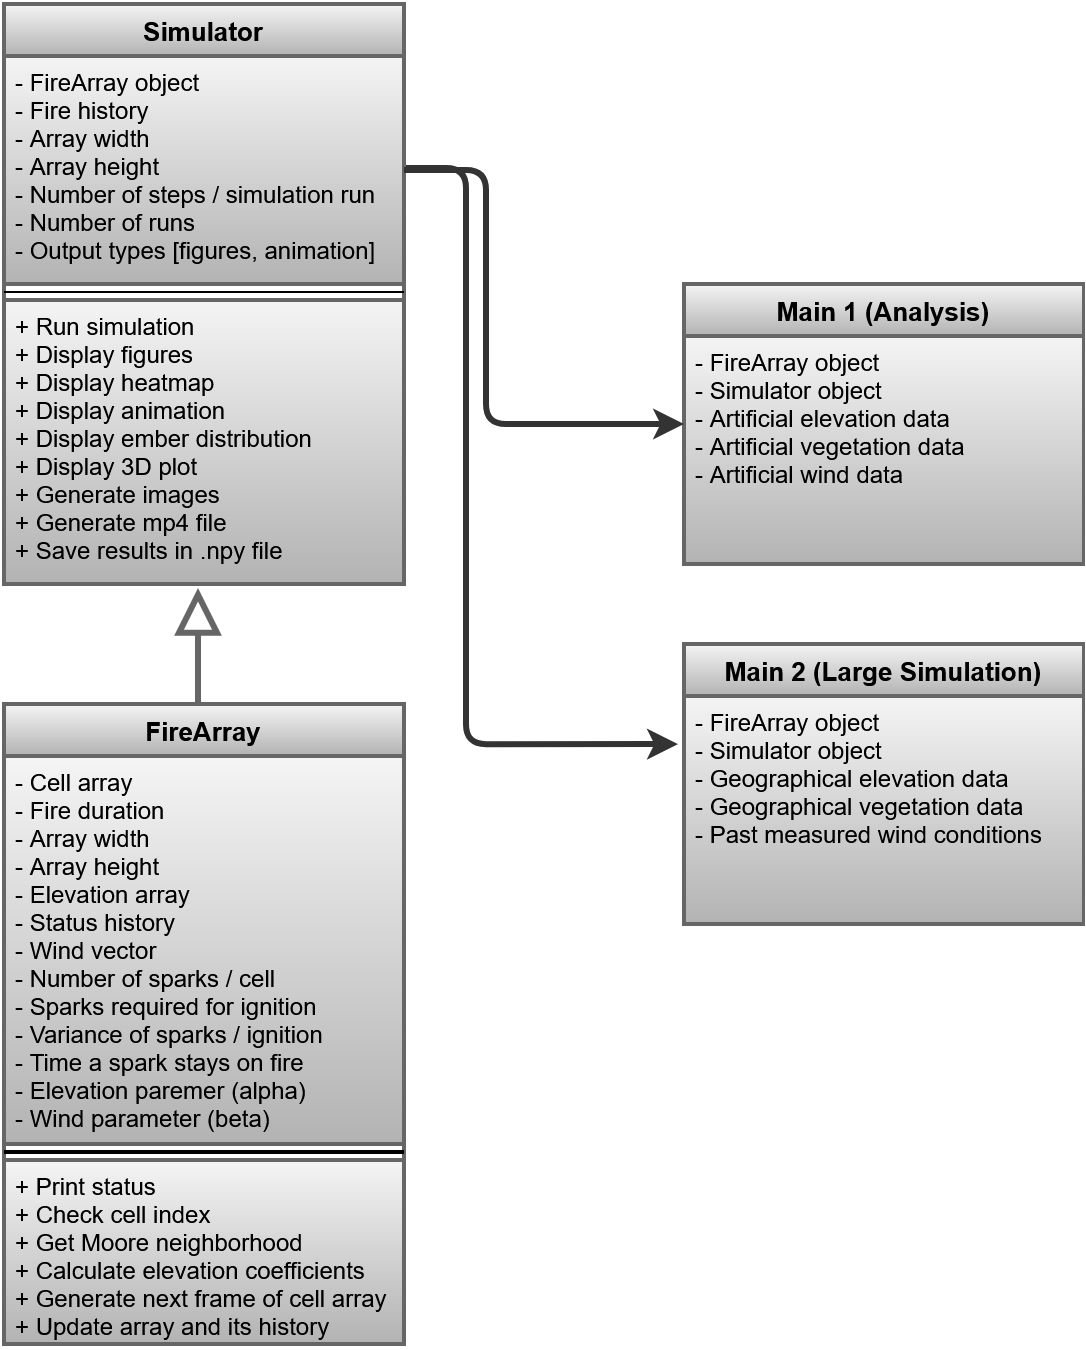
\includegraphics[width=0.8\textwidth]{Figures/FireArray.png}\caption{Class diagram for simulation code. The program is run using instances of FireArray objects, which represent the cellular automaton. The simulation and its outputs are handled by the class Simulator, which is controlled by the user via programs Main 1 and Main 2.}
\end{figure}

\section{Population Study Detail}\label{population_appendix}

Our primary motivation in understanding population behaviour is to identify the key attributes for the preservation of life. Modelling human behaviour is notoriously difficult as no two people will have the exact same reaction in a given scenario. Hence to build a relatively accurate model, one must make a series of assumptions. The fight or flight instinct was used heavily as a basis for decision making. Proportions of fight or flight populations were assimilated from 4.2.5 in J. Handmer \textit{et al.} \cite{J_Handmer}, note that this data was normalised as some populants conducted more than one key action.

\begin{figure}[h!]
    \centering
    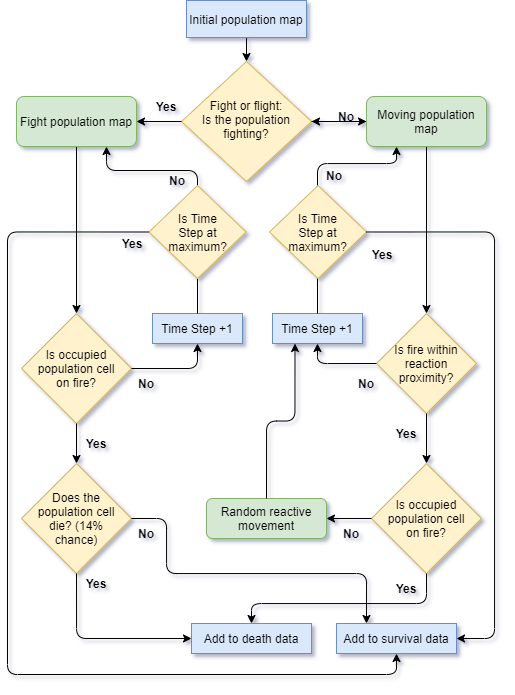
\includegraphics[width=0.65\textwidth]{Figures/population_flow.png}
    \caption{A flow chart depicting the general code decision making process for the population model. This code was able to take an initial population density map and conduct iterations up to a maximum time step. All of the deaths in the simulation were stored with the time, location and action at the time of death. This data could then be used for analysis.}
    \label{population_flow}
\end{figure}

The 'fighting' and 'flighting' populations were split and run simultaneously with the fire simulation. Fighting populants were given a 14\% probability of death if they occupied the same cell as an active fire, this mark was also determined from 4.2.5 in J. Handmer \textit{et. al}. Flighting or 'moving' populations were set up to detect fire in 4 separate cardinal regions (SE,NE,SW,NW) within a given proximity. Based on which regions detected a fire, a random reactive movement within a Moore neighbourhood resulted so that the populant would move in a general direction away from the fire(s). A summary of the coding process is offered in figure \ref{population_flow}.

\begin{figure}[h!]
    \centering
    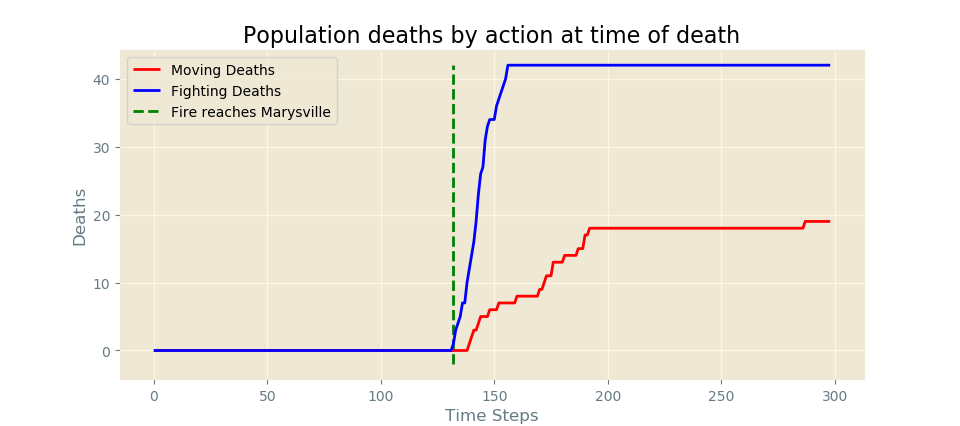
\includegraphics[width=1.0\textwidth]{Figures/fight_vs_flight_deaths.png}
    \caption{A comparison of deaths as a result of populations fighting the fire or moving away from the fire. An initial population of 500 was used with focused density at the location of Marysville. The fire simulation used had parameters of wind and elevation included.}
    \label{forf}
\end{figure}
Upon scrutiny of the data obtained, it was clear that the fighting group were at a higher risk of fatality than the moving group. This is displayed in figure \ref{forf} and is in adequate agreement with J. Handmer \textit{et. al} data. Given this understanding we can begin to present a motive to not fight a fire.
\begin{figure}[h!]
    \centering
    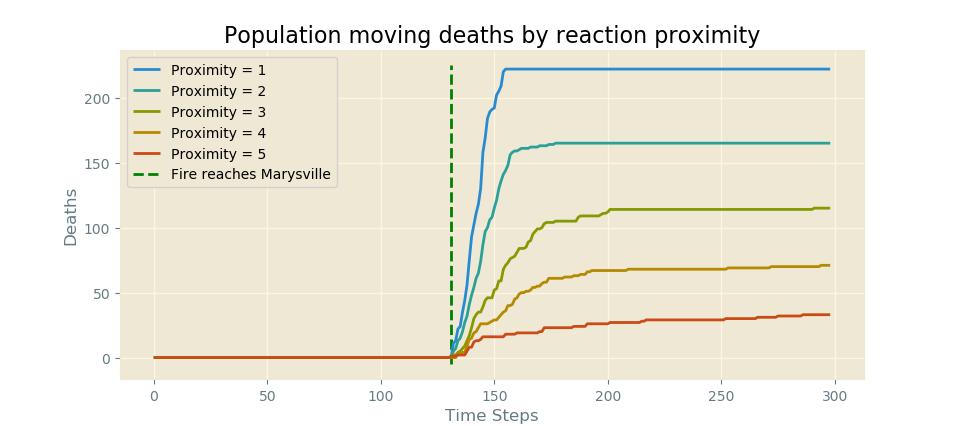
\includegraphics[width=\textwidth]{Figures/proximity_deaths.png}
    \caption{A comparison of moving deaths as a result of varying cellular reaction proximities. The same initial conditions were used as in figure \ref{forf}. The cardinal reaction regions were set square to reduce computational effort. Maximum deaths (\textit{i.e.} all of the moving population) occurred at a proximity of 1.}
    \label{proximity_deaths}
\end{figure}
A further interesting comparison is the effect of reaction proximity on death rate. Figure \ref{proximity_deaths} supplies another clear observation that the larger the reaction proximity (\textit{i.e.} the distance at which a fire needs to be in order to cause a populant to move), the higher the survival rate. This highlights the importance of making sure that populants evacuate as soon as the risk is near. This is a key finding of the Victoria Royal Bushfire Commission - 'leaving early is [still] the safest option'. \newpage \noindent In conclusion there is a lot to be learned from studying cellular automata fire-population models with the potential promise of offering life saving advice and techniques. As a direct result of the 2009 Australian bushfires, the Victorian Royal Bushfires Commission reviewed their 'stay or go' policy \cite{RoyalCommission} as it was found that it was not effective for the scale of fire experienced on Black Saturday. Modern methods now include SMS\footnote{SMS (also know as text messaging) is a mobile phone service that conveys specific messages between devices.} warnings of nearby bushfires in order to maximise survivability. Unfortunately these changes came too late for the 173 people who died in the 2009 Australian Bushfires, demonstrating the importance of such modelling.

\clearpage

\section{Project Management}\label{management}
This section contains the project plan, a Gantt chart for the projects planned progression and a complete record of all meeting agendas and minutes. The Project Plan was written at the beginning of the project to determine general objectives for the group. The agendas and minutes for meetings were recorded throughout the project.
\subsection{Project Plan}

\small

\hspace{\parindent}\textbf{Timetable}: Lent Term W11-20 \hspace{1cm} \textbf{Members}: Joonas, Joe, Antony, Alex

\textbf{Project Objectives}
\begin{itemize}
    \item Physical Background:\begin{itemize}
        \item Simulate the bushfires taking place in South-eastern Australia over the events of Black Saturday using cellular automata models.
        \item Display the evolution of the fires in the region of Murrindindi, Victoria, focussing on the town of Marysville
        \item Compare the simulation results with real data over how the fires evolved and their impact on the area and its inhabitants 
        \item Utilise real-world geographical and weather data as basis for the simulation
    \end{itemize}
    \item The Code: \begin{itemize}
        \item Writing an object-oriented program for CA simulation, using NumPy arrays and MATLAB for data acquisition
        \item Output: data about fire spread, area burnt, casualties and survivors, probability distributions of damage over critical areas
    \end{itemize}
    \item Physics Questions: \begin{itemize}
        \item Investigating how well the CA approach works as a physical model, compared to analytical alternatives such as diffusion models.
        \item Determine parameters which impact the fire damages the most
        \item Quantify the dependency of the model on physical parameters such as:
        \begin{itemize}
            \item Fire type (grass fire, bushfire, canopy fire)
            \item Fuel load (bark, leaf litter, grass etc.) \& fuel moisture
            \item Weather: wind speed \& direction, ambient temperature, relative humidity
            \item Geographical: slope angle, terrain type, water presence
            \item Barriers (water, concrete, human infrastructure)
        \end{itemize}
    \end{itemize}
    \item Resources:
    \begin{itemize}
        \item \url{https://www.ga.gov.au/scientific-topics}
        \item \url{https://en.wikipedia.org/wiki/Black_Saturday_bushfires}
        \item \url{https://en.wikipedia.org/wiki/Kinglake,_Victoria}
        \item \url{https://en.wikipedia.org/wiki/Marysville,_Victoria}
        \item \url{https://en.wikipedia.org/wiki/Shire_of_Murrindindi}
    \end{itemize}
\end{itemize}

\begin{figure}[H]\label{ganttchart}
\centering
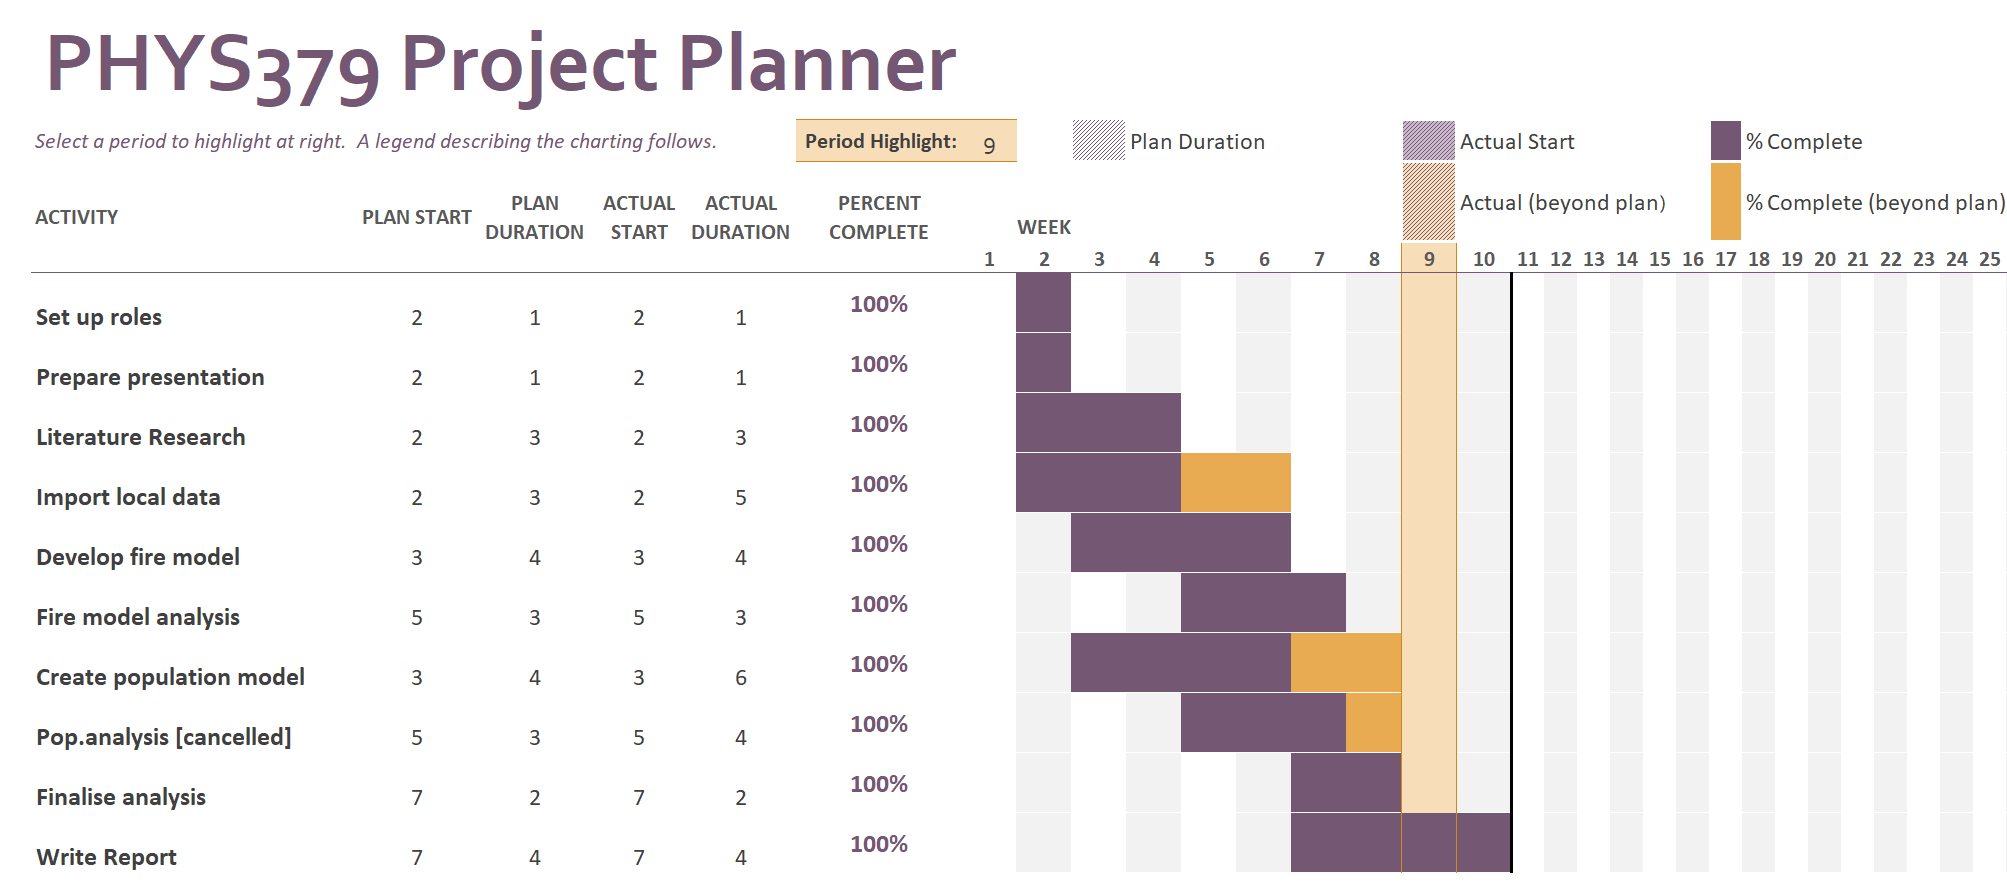
\includegraphics[width=\textwidth]{Figures/gantt_chart.png}\caption{Gantt Chart for group project, generated on 12/03/2020}
\end{figure}

\subsection{Meetings}

\subsubsection*{Week 2 Agenda \& Minutes}

\textbf{Meeting 1}

\noindent Location: Physics Building\newline
Date: 22/01/2020\newline
Time: 10:00\newline
Attendees: Joonas, Joe, Antony\newline
Apologies: Alex (TBC) 

\noindent\textbf{Agenda:}

\begin{itemize}
    \item  Assigning Roles - Set up and officiate roles for all group members: Coordinator = Joonas, Secretary = Joe.
	\item Splitting Work - Delegating each member for a specific task for next week: literature research, coding, data acquisition: split the project in 2 directions Joonas: maps, Joe: fire research, Antony: populations
	\item Project Plan - Signing and agreeing on the project plan, reading it together and making any changes
	\item Finalize Gantt chart - Set up milestones in the project and determine the general objectives 
	\item Discuss challenges - Discuss members’ coding abilities: determine easy/doable/hard tasks and assign them
	\item Common OneDrive - Set up a shared OneDrive folder for all common files: make sure all have access
	\item Additional info: Alex has not yet responded, waiting for reply
	\item Next Meeting: 28/01/2020, 10am @Physics
\end{itemize}
\clearpage
\noindent \textbf{Minutes:}

\noindent Joonas and Joe were appointed as chair and secretary respectively. The possibility of having a team name was discussed however no name was decided upon. The constitution was agreed upon and signed by Joonas, Joe and Antony. Ideas relating to the Australia Bushfire model were discussed. These ideas included: Modelling how the fire spreads throughout Australia; modelling how the population of trees and plant life were affected as the fire spread; modelling how the populations of both wild animals and humans were affected as the fire spread. Tasks were delegated for each attendee to attempt before the next meeting:  

\begin{itemize}
    \item Joonas - Creating a map of Australia of a cellular automata grid using MATLAB. 
    \item Joe – Research into how fire can be modelled using Cellular Automata. 
    \item Antony - Research into how movement of populations can be modelled using CA. 
\end{itemize}

\noindent \textbf{Meeting 2}\\
Location: In-Class, Man. LT 06\\
\noindent The project aim was discussed for the first time as a whole group. The unlikeliness of being able to create a cellular automata model containing the whole map of Australia was discussed. Possible alternative models were considered. Possible data that could be extracted from the model was also considered.  Tasks for the next meeting were updated: 

\begin{itemize}
    \item Joonas – Using maps of Australia to attempt to create a CA grid containing Australia 
    \item Joe – Finding literature to understand how fires spread and the effect of wind on their spread
    \item Alex – Creating initial code that can model fire 
    \item Antony – Finding literature to understand the movement of populations due to a large scale fire as well as fire prevention techniques
\end{itemize}

\subsubsection*{Week 3 Agenda \& Minutes}

\noindent \textbf{Meeting 3}\\
Location: Physics Building\newline
Date: 28/01/2020\newline
Time: 10:00\newline
Attendees: Joonas, Joe, Alex, Antony

\noindent \textbf{Agenda:}

\begin{itemize}
    \item Progress - Each member discussing their progress with the tasks given in the last meeting. Joonas: maps, Joe: research, Anthony: populations, Alex: N/A 
	\item Code - Group members to show progress with designing code for the project: split the task of coding into packages (ex. Fire, forest, wind, people…) 
	\item Gantt Chart - Update Gantt chart 
	\item Presentation Preparation - Designing a presentation in preparation for Thursday. Designating a particular topic to each member to rehearse for the presentation. 
	\item Future Work - Designate new tasks and goals to each member to attempt before next meeting. 
	\item OneDrive - Uploading any useful literature found by group members: Joonas to set up a folder on OneDrive 
	\item Next Meeting: Thursday 30/01 11:00
\end{itemize}

\textbf{Minutes:}

Alex was added to the shared OneDrive. Current progress with assigned tasks was discussed:

\begin{itemize}
    \item Antony – Literature on movement of populations and fire prevention techniques discussed
    \item Joe – Basic fire simulations from other sources were shown and literature on other fire simulations was discussed
    \item Joonas – His code for 1D automata and ‘Conway’s game of life’ was discussed
    \item Alex – His coding for a fire simulation was discussed
\end{itemize}

Gantt chart was updated to show the current progress of the project. Tasks to attempt during the next week were delegated:

\begin{itemize}
    \item Joe – Find data that will help make the model as realistic as possible, for example foliage cover certain parts of Australia
    \item Antony – Continue research and find parameters relating to population and fire prevention that could be added to the code
    \item Alex – Continue attempting to code fire simulations
    \item Joonas – Continue coding and attempt a simulation of fire
\end{itemize}

A group PowerPoint was created in preparation for Thursday was created and sections of the powerpoint were given to each member of the group:

\begin{itemize}
    \item Joe – Introducing the project
    \item Alex – Discussing how we aim to code a fire simulation
    \item Antony – Discussing population movements and preventative measures 
    \item Joonas – The difficulties of coding and the Gannt chart
\end{itemize}

A folder was created on the OneDrive so that any useful literature can be uploaded there.

\subsubsection*{Week 4 Agenda \& Minutes}
\noindent \textbf{Meeting 4}\\
Location: Physics Building\newline
Date: 04/02/2020\newline
Time: 15:00\newline
Attendees: Joe, Joonas, Alex, Antony

\noindent \textbf{Agenda:}
\begin{itemize}
	\item Progress - Each member discussing their progress: Joonas: fire code, Joe: geographical data, Antony: parameters for population/prevention model, Alex: fire code  
	\item Simulation plan - Joonas to explain the class structure of the CA code, determine aspects for each member to contribute to (wind, populations, etc) 
	\item Research questions - Members to come up with a physics question to answer in their investigation (ex. CA model vs diffusion, chaotic behavior, quantifying how well the model fits with physical laws [Symbol] stuff for report) 
	\item Define Objectives - Fire Simulation: \begin{itemize}
		\item Choose specific area, resolution and time for comparison (ex. Snowy Valley, 10,000 x 10,000 as hard target, town of Mallacoota 500 x 500 as easy target) 
		\item Populations \& Prevention: Antony to lead on this
		
		\item Physical parameters: 
		\begin{itemize}
			\item Grassfires vs bushfires vs canopy fires 
			\item Fuel load (bark, leaf litter, grass etc.) \& fuel moisture 
			\item Weather: wind speed \& direction, ambient temperature, relative humidity 
			\item Geographical: slope angle, terrain type, water presence 
			
			Analytical methods: someone to study how CA compares to other methods of fire modelling, maybe analytically?
		\end{itemize}
	\end{itemize}
	\item Next Milestones - Each member to commit to a deliverable for next week 
	\item Next Meeting: Thursday 06/02 1:30
\end{itemize}

\noindent \textbf{Minutes:}

The current progress of each group member’s assigned tasks was discussed:

\begin{itemize}
    \item Joe – Geographical data found during research was shown and explained to the group. Links to this data was uploaded to the OneDrive. Journals containing rules for automata when modelling fire were shown and then uploaded to OneDrive. Some research into mathematical models of wildfire not using cellular automata were discussed.
    \item Joonas – Python code that will be used for the simulation was shown and the class structure within the code was explained. This code was then used to show a fire simulation. Complications such as speed of run time with the code were discussed. Joonas explained how the data found by Joe could be implemented into the code.
    \item Antony – Flow chart showing how a population would react in the event of a wildfire was explained and discussed. Population data (how many people would leave etc.)  found during research was discussed. Ideas of how to code the movement of populations were then discussed.
    \item Alex – Progress with coding of fire simulation was discussed. Papers containing information about modelling wind were discussed.
\end{itemize}

\noindent Tasks to attempt in the next week were delegated. Group members should think of a physics question to answer in their investigation which could be mentioned in the final group report. As well as this each member should attempt to find data on a specific location that our simulation could be used to model. Individual tasks for the next week were:

\begin{itemize}
    \item Joe – Create short report on the different types of analytical modelling approaches. Use MATLAB to get geographical data into useable format.
    \item Joonas – Rewriting the simulation code such that it can be ran in a shorter time. Use MATLAB to get geographical data into useable format.
    \item Antony – Using literature on population movements to create some code that models a population. Use MATLAB to get geographical data into useable format.
    \item Alex – Create a 2D wind automaton and find useable data on wind speeds etc. 
\end{itemize}
\clearpage

\subsubsection*{Week 5 Agenda \& Minutes}
\textbf{Meeting 5}\newline
Location: Physics Building\newline
Date: 11/02/2020\newline
Time: 15:00\newline
Attendees: Joonas, Joe, Antony, Alex

\noindent\textbf{Agenda:}
\begin{itemize}
    \item Progress - Each member discussing their progress. Joonas: code \& geographical data, Joe: research on analytical approaches, Alex: wind model, Antony: code on population movement
    \item Simulation plan @Joonas - Confirm final parameters for fire model, to be programmed. Joonas: topography is doable within a week; fire hopping will take another (and will significantly affect runtime).
    Data acquisition: need a specific physical area to investigate. TBC during meeting, so that everyone can investigate the topic.
    \item Geographical Data @Joonas - Obtaining readable input data for simulation is crucial. Detailed elevation data is required, as well as data on flammable / non-flammable terrain. This will require information on vegetation cover, where a fixed threshold / criterion is needed to determine how flammable a cell is.
    \item Population Model @Antony - Status update: What is a realistic objective for this? What is the status of the code?
    \item Wind Model @Alex - Status update: is wind data possible to incorporate to the simulation within the timeframe?
    \item Analytical Methods @Joe - Report on the subject?
    \item Next milestones - Each member to commit to a deliverable for next week
    \item Next Meeting: Thursday 13:00
\end{itemize}
\textbf{Minutes:}

Current progress with each group members designated tasks were discussed:
\begin{itemize}
    \item Joonas – The current progress of the main fire simulation code was explained and discussed. The code was shown to the rest of the group and Joonas explained how the code has been altered to run faster and be easier to use. Joonas then explained how the code handles fire when it reaches the end of the automata grid as well as the how the rules implemented in the code were the same as those used by Quartieri in 2014. Joonas explained how the vegetation data from ‘Geoscience Australia’ was used within the code.
    \item Joe – Despite having difficulties In downloading MATLAB, Joe has now gained access to MATLAB so is able to begin processing data. Joe explained the data he has found on the ‘Black Saturday’ fires in 2009 and how we could use this within our project. Joe then explained the different types of analytical methods involved with wildfire and showed the beginning of his report of the subject.
    \item Antony – The data Antony found during his research on the ‘Black Saturday’ fires was explained and its usefulness was discussed. Antony has also downloaded MATLAB in preparation for processing data. Antony explained the current form of his code for the movements of populations as a result of fire. Antony explained how his code correctly shows that populations respond as a result of fire however the mechanisms by which these populations move (move away from the fire) are not yet correct.
    \item Alex - The current progress of Alex’s simulation for the wind model was discussed. Alex explained issues relating to the model such as run time due to the extremely large amount of win data available for the whole of Australia. Boundary conditions for the win model were then discussed.
\end{itemize}

\noindent Further plans for improving the current fire simulation code were then discussed. These plans included features such as topography and fire hopping. The big issue of dealing with long run times were then discussed. It was decided that we should aim to simulate a smaller area than initially planned. The area decided on was Marysville, Victoria. It was decided that during the next week, whilst Joonas is updating the fire simulation code, that Alex, Joe and Antony should attempt to find as much geographical data relating to Marysville as possible; this would include wind data, elevation data etc ideally in .shp file. In preparation for next week Antony and Alex should also continue their respective coding tasks and Joe should finish his report on analytical methods.
\subsubsection*{Week 6 Agenda \& Minutes}
\textbf{Meeting 6}\newline
Location: Physics Building\newline
Date: 18/02/2020\newline
Time: 15:00\newline
Attendees: Joonas, Joe, Antony, Alex

\noindent \textbf{Agenda:}
\begin{itemize}
    \item Progress - Each member discussing their progress. Joonas: updates on fire code, Joe: report on analytical approaches, Alex \& Antony: code on population movement.
    \item Simulation plan @Joonas - Topography has been implemented. (Example to be shown) Next steps: Joonas can add wind within a week but hopping will most likely be too time-consuming. Proposal: Joonas to work on finding data from Marysville as is, and running simulation using the data.
    \item Side note on wind @Joonas - Alex’s wind data was analysed and imported into MATLAB. Issue encountered: no directional information was found. Confirmation from @Alex?
    \item Population Model @Antony - Status update: state of the code now, required inputs, desired outputs, parameters to analyse?
    \item Analytical methods \& data analysis @Joe - Report on the subject to be shown. Discussion and analysis of fire behaviour with model V3.
    \item Publishing data @Joonas - The data generated by FireModel to be uploaded on OneDrive so that others can access it. This includes .npy files containing the fire evolution, for use in the population model of @Alex and @Anthony 
    \item Next Milestones - Each member to commit to a deliverable for next week.
    \item Next Meeting: Thursday 13:30
\end{itemize}
\textbf{Minutes:}

The progress of each group member from the past week was discussed:
\begin{itemize}
    \item Joonas – The final fire simulation python code is almost finished. Joonas explained the different parameters that have been implemented into the code such as wind and elevation etc and how they can be controlled within the code. Joonas explained how fire hopping affected the data produced by the simulation and the run time. The wind data that has been used in the code was discussed as it lacked data for the direction of the wind. Joonas also explained the method he has used to create a 3D movie of the simulation (this was shown to the rest of the group) and the remaining bugs that he needed to fix.
    \item Antony and Alex – Good progress has been made with coding the movement of populations. Antony and Alex explained the basic premise behind how the code works, this includes a detection region that will dictate how a cell will move in a time step. Ideally this code will eventually produce an animation however it currently just produces data. This code will use the data produced by Joonas’ fire code as an input. Joonas has sent an example of this data. Currently the detection region used in this simulation is square however this may be changed to be spherical at a later data. Other issues that need to be considered within this code such as maintaining the correct population number were discussed. Alex explained how the data for the wind would best be used over a small area such as Marysville (direction won’t change considerably).
    \item Joe – Joe explained the format of his first draft of the ‘Analytical methods in modelling wildfire’ report and the important conclusions from it. This will be uploaded to the OneDrive and will be developed further during the coming week. Joe then explained some of the data analysis that he had been conducting on version 3 of Joonas’ fire simulation code. Firstly, Joe discussed the effects of: starting the fire in a different location on the grid; changing the location of non-fuel cells; changing the duration of the fire cells etc. Joe explained the how the results of numerous runs of the simulations vary due to the probabilistic nature of the code and how this forms a distribution of results. Further analysis of what type of distribution this is will be conducted; Joonas proved some ideas as to how this could be done in an easier way. 
\end{itemize}

\noindent Tasks to be attempted for the next week were delegated: Joe will continue analysing the different versions of Joonas’ code; Joonas will fix the current bugs in the latest version of code before uploading it to the OneDrive as well as finding useable data on Marysville; Antony and Alex will finish the population model so it is ready for analysis.

\subsubsection*{Week 7 Agenda \& Minutes}
\textbf{Meeting 7}\newline
Location: Physics Building\newline
Date: 25/02/2020\newline
Time: 15:00\newline
Attendees: Joonas, Joe, Antony\newline
Apologies: Alex

\noindent \textbf{Agenda:}
\begin{itemize}
    \item Progress Update @All - Joonas: code 100\% complete, data obtained from Marysville. Joe: fire model analysis, Alex \& Antony: analysis on population model. Is population model ready by now? What does the data look like?
    \item Simulation plan @Joonas - Joonas to find initial conditions of Murrindindi fire and run simulations on the data obtained.
    \item Fire Model Analysis @Joe - Results from code to be described: a briefing on main observations. List of things to investigate by next meeting
    \item Report writing @All - Begin writing report: assign sections for each member. Shared Overleaf document has been created for this purpose. Proposal by Joonas: \begin{itemize}
        \item Introduction by Joe \& Antony: general wildfire info \& motivation for modelling a system using CA ({\raise.17ex\hbox{$\scriptstyle\sim$}}2 pages)
        \item Background of CA modelling by Joe, review of past literature ({\raise.17ex\hbox{$\scriptstyle\sim$}}2 pages)
        \item Methodology: principles of modelling fire \& code flowchart by Joonas, population model by Alex ({\raise.17ex\hbox{$\scriptstyle\sim$}}3 pages)
        \item Results part I: physical accuracy of fire model \& quantifying fire behaviour by Joe ({\raise.17ex\hbox{$\scriptstyle\sim$}}4 pages)
        \item Results part II: simulation results using real-world data by Joonas ({\raise.17ex\hbox{$\scriptstyle\sim$}}3 pages)
        \item Results part III: Antony and Alex on population model \& its results ({\raise.17ex\hbox{$\scriptstyle\sim$}}3 pages)
        \item Conclusion by Antony ({\raise.17ex\hbox{$\scriptstyle\sim$}}2 pages)
        \item Appendices: Joe (to include project plan, agendas and minutes)
    \end{itemize}
    \item Next Milestones - Each member to commit to a deliverable for next week. Timeframe of report to be agreed upon, writing to begin.
    \item Next Meeting: Thursday 13:30
\end{itemize}
\textbf{Minutes:}
Current progress with designated tasks of each present member of the group was discussed:
\begin{itemize}
    \item Joonas – The final version of the code has been fully debugged and sent to each group member for analysis (Joe). The required data for the area of Marysville, including elevation etc, has been found and implemented into the code.  Despite the fact that no vegetation data for 2007 could be found, this is not an issue. Joonas has run the simulation fully (this required 8 hours in total), and the results were shown to the group and discussed. Joonas discussed his plans to analyse the code in terms of how well it can model Australian bushfires and how it can be compared to empirical data from the bushfires.
    \item Joe – Analysis conducted since Thursday was shown and discussed. This included : analysis into how the percentage of fire with in the automata grid varies over time and how different factors such as wind and elevation effect this; quantitative analysis into the effect of changing the elevation coefficient alpha on the percentage of fire over time; the value of alpha at which the effect of elevation was completely dominant; quantitative analysis into the effect of changing the wind coefficient beta on the fire spread and the value at which beta becomes dominant. Joe expressed issues with the mechanism of fire spreading within the code however this issue has since been resolved. Joonas provided assistance into why some of Joe’s analysis methods were not working.
    \item Antony – Data found on the populations within Marysville was discussed; there were issues with finding an exact value for this as Marysville is tourist spot so the actual population can vary. This may also make it difficult to use the model to model the movement of populations and the number of deaths etc. Antony went through and discussed some papers of the reactions of populations to wildfire and how they have been implemented into the code. The code that Antony and Alex have been working on has made great progress and is now almost finished, this was shown to the rest of the group. Joonas has shown how the data produced by his fire model can be inputted into the population code. Future plans for this code were discussed.
\end{itemize}

The plans for the report that Joonas outlined in the agenda were discussed and agreed upon. Each member was happy with what they needed to write for the report. Tasks for next week were decided: Joe will continue his analysis into the theory of the code; Joonas will begin analysis into how well the code models the Australian bushfires and compare this to real data; and Antony will finish his population code with Alex.   

\subsubsection*{Week 8 Agenda \& Minutes}
\textbf{Meeting 8}\newline
Location: Physics Building\newline
Date: 03/03/2020\newline
Time: 15:00\newline
Attendees: Joonas, Joe, Antony, Alex

\noindent \textbf{Agenda:}
\begin{itemize}
    \item Progress Update @All - Joonas: writing started, Marysville simulations inconclusive. Report writing started: everyone has been added to Overleaf. Joe: writing started, model analysis complete. Antony \& Alex: population model?
    \item Model Analysis @Joe - A briefing of results obtained from fire model.
    \item Report @Joonas - Flow chart added to report, as well as two figures on Marysville. Section on methodology in progress, to be completed by the end of the week, as well as section on modelling Marysville region fires (Results part II).
    \item Report @Joe - Introduction to wildfire modelling, and motivation. Background of CA modelling, review of past literature. Results part I: physical accuracy of fire model \& quantifying fire behaviour. Appendices to include project plan, agendas and minutes.
    \item Report @Antony - Population model description and discussion of past literature, results and discussion (Results part III), conclusion
    \item Report @Alex - Methodology used in population model
    \item Presentation W10 - Allocate tasks / slides to do for week 10 presentation
    \item Next Milestones - Deadlines for chapters on report to be set and agreed upon.
    \item Next Meeting: Monday 13:30
\end{itemize}
\textbf{Minutes:}
\begin{itemize}
    \item The format of the final report and what each section of the report will contain was discussed. It was discussed how the population should feature in the report. It was decided that the population model will be mentioned in the ‘Future works’ section of the report and then analysed in detail in the appendix of the report. How the minutes and agendas of each meeting should be integrated into the report was decided; they will be copied from their word documents and pasted into overleaf as opposed to uploading them as pictures.  The team name of ‘Wombats on fire’ was decided upon for admin reasons such as when filling out the peer assessment forms etc. Joonas then discussed the current progress of his analysis.\newline
    \item Joonas found that due to a rapid wind change during the ‘Black Saturday’ bushfires that it would be incredibly difficult to model the spread of fire over Marysville. This means that some of the data from this simulation is inconclusive. Possible solutions to this issue were discussed however none were feasible in the time remaining to complete the project. Some of the animations produced by Antony and Alex’s population model were shown. This code is now without any known bugs. Joe explained his analysis and it was discussed with the group. Joe’s plan to generate an equation that accurately describes the probability of a cell being on fire and the dependence of this on a variety of parameters was discussed was explained and discussed. Joe explained the sections of his report that he has written so far (background and beginning of analysis section). \newline 
    \item Tasks for each group member for the were designated: Joe will create his probability equation and finish his sections (background and analysis) of the report; Joonas will finish writing his sections (methodology and analysis) of the report; Antony will write the introduction of the report and provide comments on the sections written by Joe and Joonas, as well as  create the presentation slides for the week 10 presentation; Alex will put all the project planning documents in the appendix of the report and help Antony prepare the presentation slides.
\end{itemize}

\subsubsection*{Week 9 Agenda \& Minutes}
\textbf{Meeting 9: Last Official Meeting}\newline
Location: Physics Building\newline
Date: 09/03/2020\newline
Time: 14:00\newline
Attendees: Joonas, Joe, Antony, Alex

\noindent \textbf{Agenda:}
\begin{itemize}
    \item Report @Joonas - Methodology, Analysis on Marysville \& Future Work completed.
    \item Report @Joe - Background \& Analysis of Fire Model in progress: updates?
    \item Report @Antony - Feedback to others, Intro \& Conclusions. Updates?
    \item Report @Alex - Appendices: Minutes, Agendas \& Project Plan. Updates?
    \item Presentation W10 - When will slides be ready? Which figures want to use? Practice run to be done with the whole group before presentation?
    \item Next Milestones - Deadlines on report: full draft to be submitted to Ed by Thursday 14:00.
    \item Next Meeting: Monday 16th @11:00
\end{itemize}
\textbf{Minutes:}

Updates on current progress of report and what needs doing: 
\begin{itemize}
    \item Joonas’ methodology and analysis sections have been completed. Joonas will now write the conclusion of the report to give Antony more time to write the feedback. 
    \item Joe’s background and analysis sections have been completed. 
    \item Antony will read through the report and add comments and feedback on how it can be improved and made more similar to Ed’s template on Moodle. Antony will write the introduction to the report.
    \item Alex will upload copies of the project plan, agendas and minutes to the appendices of the report.
\end{itemize}
Ideally the report will be completely written by Thursday so that Ed can give feedback on the whole thing.
A discussion into the specific motivation for our project was discussed, however no decision was made.
Finally, it was decided that Joe and Antony will make the presentation slides for the presentation on Monday.